\documentclass[11pt,letterpaper]{article}
\usepackage[utf8]{inputenc}
\usepackage[top=1in,bottom=1in,left=1in,right=1in]{geometry}
\usepackage{amsmath}
\usepackage{amsfonts}
\usepackage{amssymb}
\usepackage{amsthm}
\usepackage{bm}
\usepackage{braket}
\usepackage{cancel}
\usepackage{enumitem}
\usepackage{float}
\usepackage{graphicx}
\usepackage{hyperref}
\usepackage{mathabx}
\usepackage{parskip}
\usepackage{tensor}
\usepackage{titlesec}
\usepackage{titling}


\setenumerate{leftmargin=*,label=\bf(\alph*)}


\titlelabel{(\thetitle)\quad}
\titleformat*{\section}{\large\bfseries}
\titleformat*{\subsection}{\normalsize\bfseries}
\setlength{\droptitle}{-5em}

\DeclareMathOperator*{\argmin}{arg\,min}
\DeclareMathOperator*{\argmax}{arg\,max}

\let\Re\relax
\DeclareMathOperator{\Re}{Re}
\let\Im\relax
\DeclareMathOperator{\Im}{Im}


\newcommand{\bhat}[1]{\hat{\bm{#1}}}


\renewcommand{\thesubsection}{\normalsize \alph{subsection}}
\renewcommand{\d}{\mathrm{d}}
\renewcommand{\vec}[1]{\bm{#1}}
\newcommand{\del}{\vec{\nabla}}
\newcommand{\e}{\epsilon}
\newcommand{\tpd}[3]{\left( \frac{\partial #1}{\partial #2} \right)_{#3}}
\newcommand{\pd}[2]{\frac{\partial #1}{\partial #2}}
\newcommand{\spd}[2]{\frac{\partial^2 #1}{\partial {#2}^2}}
\def\dbar{{\mathchar'26\mkern-12mu d}}

\allowdisplaybreaks


\author{Sam Kowash}
\numberwithin{equation}{section}
\numberwithin{figure}{section}
\title{CSE 546 HW \#notes}

\begin{document}
\maketitle


\section{LASSO}
Selects for sparse predictor $w$. We may want this either for efficiency or human-legibility. How do we do this? Well, greedy approach adds features one at a time based on improvement in test error, but that's pretty hacky. How do we know when to stop? How do we avoid just including a billion features?

Looking for sparse results is a type of regularization; we want to penalize feature overselection. This motivates the lasso objective:
%
\begin{align}
	\hat{w}_{lasso} &= \argmin_{w} \sum_{i=1}^n \left(y_i-x_i^T w\right)^2 + \lambda \|w\|_1.
\end{align}
%
This punishes big vectors $w$, which is what we want. Fact: for any $\lambda \geq 0$ for which $\hat{w}_r$ finds the minimum, there exists $\nu \geq 0$ such that
%
\begin{align}
	\hat{w}_r &= \argmin_{w} \sum_{i=1}^n \left(y_i - x_i^T w\right)^2 \, \text{subject to } r(w) \leq \nu.
\end{align}
%
That is, regularized regression problems can always be reframed as constrained optimization.

\begin{figure}[H]
	\centering
	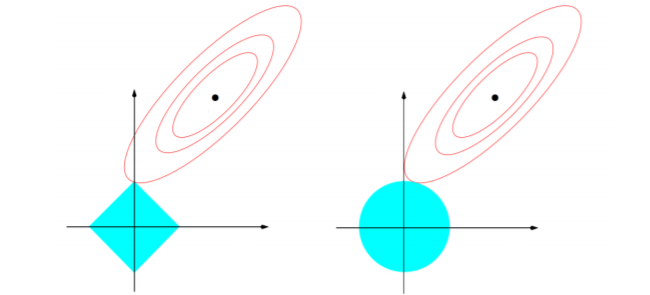
\includegraphics[width=.6\textwidth]{figures/lasso_v_ridge.png}
	\caption{Lasso on left, ridge on right; lasso prefers solutions along coordinate axes (i.e. sparse)}
\end{figure}

If we incorporate an offset,
%
\begin{align}
	\hat{w},\hat{b} &= \argmin_{w,b} \sum_{i=1}^n \left(y_i - (x_i^T w + b)\right)^2 + \lambda \|w\|_1,
\end{align}
%
but joint optimization is a pain, so let's prefer to de-mean our data. This is still actually kind of tricky minimization; the 1-norm isn't differentiable at the origin and this complicates things. Do by coordinate descent, minimize one direction at a time. This is guaranteed to approach the optimum for lasso (which is nice), but how do we pick our order of coordinate descent? Options,
%
\begin{itemize}
	\item Random each time
	\item Round robin
	\item Try to pick ``important'' coordinates (biases us).
\end{itemize}

Let's see an example. Take $j \in \{1,\ldots,d\}$.
%
\begin{align}
	\sum_{i=1}^n \left(y_i - x_i^T w\right)^2 + \lambda \|w\|_1 &= \sum_{i=1}^n \left(y_i - \sum_{k=1}^d x_{i,k} w_k\right)^2 + \lambda \sum_{k=1}^d |w_k|\\
	&= \sum_{i=1}^n \left(\left(y_i- \sum_{k\neq j} x_{i,k} w_k \right) - x_{i,j} w_j \right)^2 + \lambda \sum_{k\neq j} |w_k| + \lambda |w_j|.
\end{align}
%
So set $\hat{w}_k = 0$ for $k \in \{1,\ldots,d\}$ and loop over points:
%
\begin{align}
	r_i^{(j)} &= \sum_{k\neq j} x_{i,j} \hat{w}_k\\
	\hat{w}_j &= \argmin_{w_j} \sum_{i=1}^n \left(r_i^{(j)} - x_{i,j} w_j \right)^2 + \lambda |w_j|.
\end{align}

Pulling out one 1-d problem at a time! Works b/c lasso objective is \emph{separable}. Except\ldots this isn't actually a lot better. Hard to optimize because of pointy bit. Need to extend some concept of derivative and convexity. Traditional definition for fn is that lines b/t points on $f(x)$ lie above $f(x)$ (epigraph is convex). We need a different one here:
%
\begin{align}
	f(y) &\geq f(x) + \nabla f(x)^T (y-x) \quad \forall x,y
\end{align}
%
This amounts to saying that there's a ``supporting hyperplane'' touching the epigraph at $x$ such that the epigraph lies entirely on one side of the plane. If the function is differentiable at $x$, this is going to be the tangent plane. If not, we may have \emph{many} options, and these are called \emph{subgradients} (denoted $\partial_{w_j}$ for subgradient set at $w_j$). We call differentiable functions extremized at $x$ where $\nabla f(x) = 0$, and similarly we will call other functions extremized when $f(x)$ admits 0 as a subgradient at $x$.

OK, so how do we actually take subgradients and set them to zero? Consider example,
%
\begin{align}
	\partial_{w_j} \left(\sum_{i=1}\left(r_i^{(j)} - x_{i,j} w_j\right)^2 + \lambda |w_j|\right) &= \left\{\begin{array}{lr}
		a_j w_j - c_j - \lambda & \text{if } w_j < 0\\
		\left[-c_j - \lambda, -c_j + \lambda\right] & \text{if } w_j = 0\\
		a_j w_j - c_j + \lambda & \text{if } w_j > 0\\
		\end{array}\right.,
\end{align}
%
where
%
\begin{align}
	a_j &= \left(\sum_{i=1}^n x_{i,j}^2\right), &
	c_j &= 2\left(\sum_{i=1}^n r_i^{(j)} x_{i,j}\right).
\end{align}
%
This tells us how to do our minimization (look for regime that contains zero as subgrad):
%
\begin{align}
	\hat{w}_j &= \left\{\begin{array}{lr}
		\frac{c_j + \lambda}{a_j} & \text{if } c_j < -\lambda\\
		0 & \text{if } |c_j|\leq \lambda\\
		\frac{c_j - \lambda}{a_j} & \text{if } c_j > \lambda\\
		\end{array}\right.
\end{align}
%
where, recall,
%
\begin{align}
	a_j &= \sum_{i=1}^n x_{i,j}^2 & c_j &= 2 \sum_{i=1}^n \left(y_i - \sum_{k\neq j} x_{i,k} w_k\right) x_{i,j}.
\end{align}
%
This central flattening behavior provides ``soft thresholding''; can make predictor entries identically zero depending on strength of regularization.






















\section{Classification problems}
Different from regression! Same principles though. Need a loss function; what is? Let's start with binary classification, want to learn $f: X \to Y$ where $X$ contains features, $Y \in \{0,1\}$ is target class. Natural loss is 0/1 function: $\bm{1} \{f(X) \neq Y \}$. Expected loss is then
%
\begin{align}
	\mathbb{E}_{XY} \left[\bm{1}\{f(X) \neq Y\}\right] &= \mathbb{E}_X \left[\mathbb{E}_{Y\mid X}\left[\bm{1}\{f(x) \neq Y\} \mid X=x\right]\right]\\
	&= \mathbb{E}_X \bigg\{ \bm{1}\{f(x)=1\}\mathbb{P}(Y=0 \mid X=x) + \bm{1}\{f(x)=0\}\mathbb{P}(Y=1 \mid X=x) \bigg\}.
\end{align}
%
Supposing we know $P(Y\mid X)$, the Bayes optimal classifier is 
%
\begin{align}
	f(x) &= \argmax_{y} \mathbb{P}(Y=y \mid X=x).
\end{align}

How do we actually estimate $\mathbb{P}(Y \mid X)$? Well, can't do linear, and we're out of tricks now. Need a new trick; some function that goes from $\mathbb{R}^d$ to $[0,1]$ (called link function). A nice option is the sigmoid/logistic curve:
%
\begin{align}
	\mathbb{P}(Y=0 \mid X,W) &= \frac{1}{1+\exp\left[w_0 + \sum_i w_i X_i\right]}.
\end{align}
%
Still a sort of linear model in terms of what we do to our data variables. Note that $w_0$ applies a horizontal shift, and the $w_i$ ``stretch'' the curve. Note a nice property for binary classification, which is that
%
\begin{align}
	\frac{\mathbb{P}(Y=1 \mid w,X)}{\mathbb{P}(Y=0 \mid w,X)} &= \exp\left[w_0 + w^T X\right].
\end{align}
%
Reasonable to make our rule to classify as 1 if ratio is greater than 1, classify as 0 if ratio is less than 1. Equivalent result,
%
\begin{align}
	\ln \frac{\mathbb{P}(Y=1 \mid w,X)}{\mathbb{P}(Y=0 \mid w,X)}  = w_0 + \sum_i w_i X_i \to \left\{
		\begin{array}{l}
			< 0 \implies \text{ classify as 0}\\
			> 0 \implies \text{ classify as 1}\\
		\end{array}\right..
\end{align}

Alternative formulation (conditional likelihood): say $y \in \{-1,1\}$ instead of $\{0,1\}$ so we can then write
%
\begin{align}
	\mathbb{P}(Y=y \mid x,w) &= \frac{1}{1+\exp\left(-y w^T x\right)}
\end{align}
%
and find the MLE:
%
\begin{align}
	\hat{w}_\mathrm{MLE} &= \argmax_w \prod_{i=1}^n \mathbb{P}(y_i \mid x_i,w)\\
	\hat{w}_\mathrm{MLE} &= \argmin_w \sum_{i=1}^n \underbrace{\log\left(1+ \exp\left(-y_i x_i^T w\right) \right)}_{\sigma(y_i x_i^T w)}
\end{align}
%
Call the objective $J(w)$ (logistic loss): what the hell does it look like? Is it convex? (Yes.) How do we minimize it? Note that for an argument $z$, $\sigma(z) \sim |z|$ as $z \to -\infty$ and $\sigma(z) \to 0$ as $z \to +\infty$. In between, does some nonsense. So $\sigma(z)$ is easy to understand, but what about $J(w)$? Generally, no closed form in terms of $w$, can't just take derivative and set to zero. It turns out, moreover, that if we happen to have a $w$ that correctly classifies every point (by dumb luck; linearly separable data set), then $y_i x_i^T w$ is strictly positive and so for $t > 0$, $y_i x_i^T (tw) > y_i x_i^T w$ and we will always prefer to infinitely extend our $w$ along our ``good'' direction to continue reducing loss. This breaks the classifier. Sigmoid classifiers become step functions. We \emph{need} to regularize this conditional log likelihood objective.













\section{Gradient descent}
Recall that our general problem is to be handed i.i.d. data $\{(x_i,y_i)\}_{i=1}^n$ with $x_i \in \mathbb{R}^d$ and $y_i \in \mathbb{R}$, a model with some parameters $w$, and some loss function depending on $w$ to be calculated on our data, then optimize $w$ with respect to that loss. The computational meat is in optimization. We turn it into a problem that looks like $X^T X w = X^T Y$, but how do we actually do that? Lots of different ways! Many algorithms! Some depend on properties of matrices, sparseness, etc. Let's look at one in particular, which is gradient descent.

Say I have some function $f(x)$ where $x \in \mathbb{R}^d$. Taylor tells us that
%
\begin{align}
	f(x + \delta) &= f(x) + \nabla f(x) \cdot \delta + \cdots,
\end{align}
%
so at any point we can find the gradient and take a step in the opposite direction, which must decrease $f$. Ex:
%
\begin{align}
	f(w) &= \frac{1}{2} \|X w - y\|_2^2\\
	\nabla f(w) &= X^T(Xw -y) = X^T (Xw -y) = X^T X w - X^T y,
\end{align}
%
so if we are at some $w_t$ our next step should be
%
\begin{align}
	w_{t+1} &= w_t - \eta X^T(X w_t - y).
\end{align}
%
Examine recursion behavior, find (for optimum $w_\ast$) that
%
\begin{align}
	(w_{t+1} - w_\ast) &= \left(I - \eta X^T X \right)^{t+1} (w_0 - w_\ast),
\end{align}
%
so can bound rate of approach to optimum. (Shocker: need $\eta$ small.)


We can do one better by going one step further down the Taylor series,
%
\begin{align}
	f(y) &\approx f(x) + f'(x) (y-x) + \frac{1}{2} f''(x) (y-x)^2
\end{align}
%
make our next step the minimum
%
\begin{align}
	\tilde{y} &= \frac{f'(x)}{f''(x)}
\end{align}





\end{document}